\section{Ejemplos de los resultados}
A continuación, se muestra un ejemplo de cada uno de los resultados obtenidos de la simulación de los módulos obtenidos de las 3 síntesis: \code{RTLIL}, \code{cmos\_cells.lib}, y \code{cmos\_cells.lib} con retardos.
Además, se utlizó el archivo \code{wave\_names.ttf} (Translate Filter File) para mostrar el nombre de cada señal en las formas de onda, lo cual facilita la lectura de las mismas.

Como punto de comparación, a continuación se muestra la forma de onda obtenida para la simulación del módulo conducutal de la Tarea \#1:

\begin{figure}[!h]
    \centering
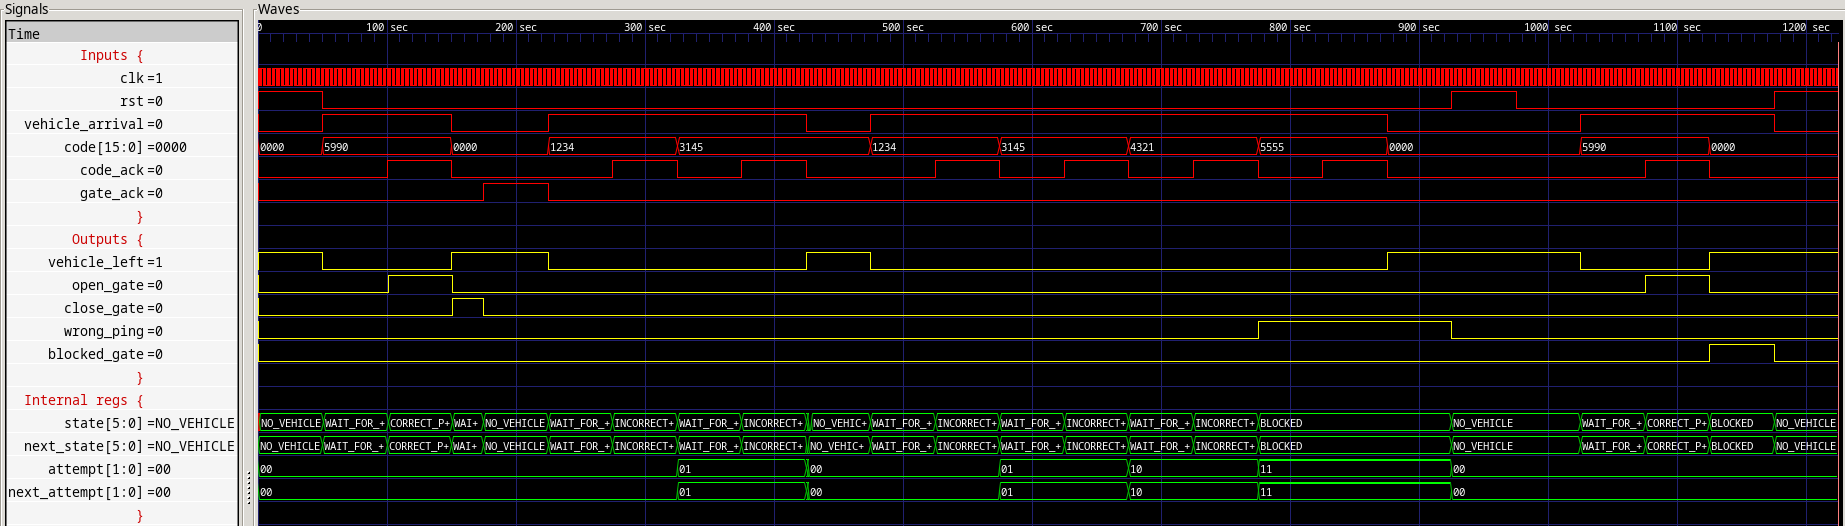
\includegraphics[width = 1\linewidth]{figs/sim.png}
\caption{Forma de onda de la simulación del módulo conductual \code{behavioral\_parkingController}}
    \label{behavioral}
\end{figure}

Ya se comprobó en la Tarea \#1 de que esta forma de onda da como resultado el comportamiento esperado para el módulo, por lo que se compararán las formas de onda mostradas en las secciones a continuación con esta para verificar el funcionamiento adecuado de los módulos sintetizados.

\newpage

\subsection{RTLIL}
Se obtuvo la siguiente forma de onda:

\begin{figure}[!h]
    \centering
    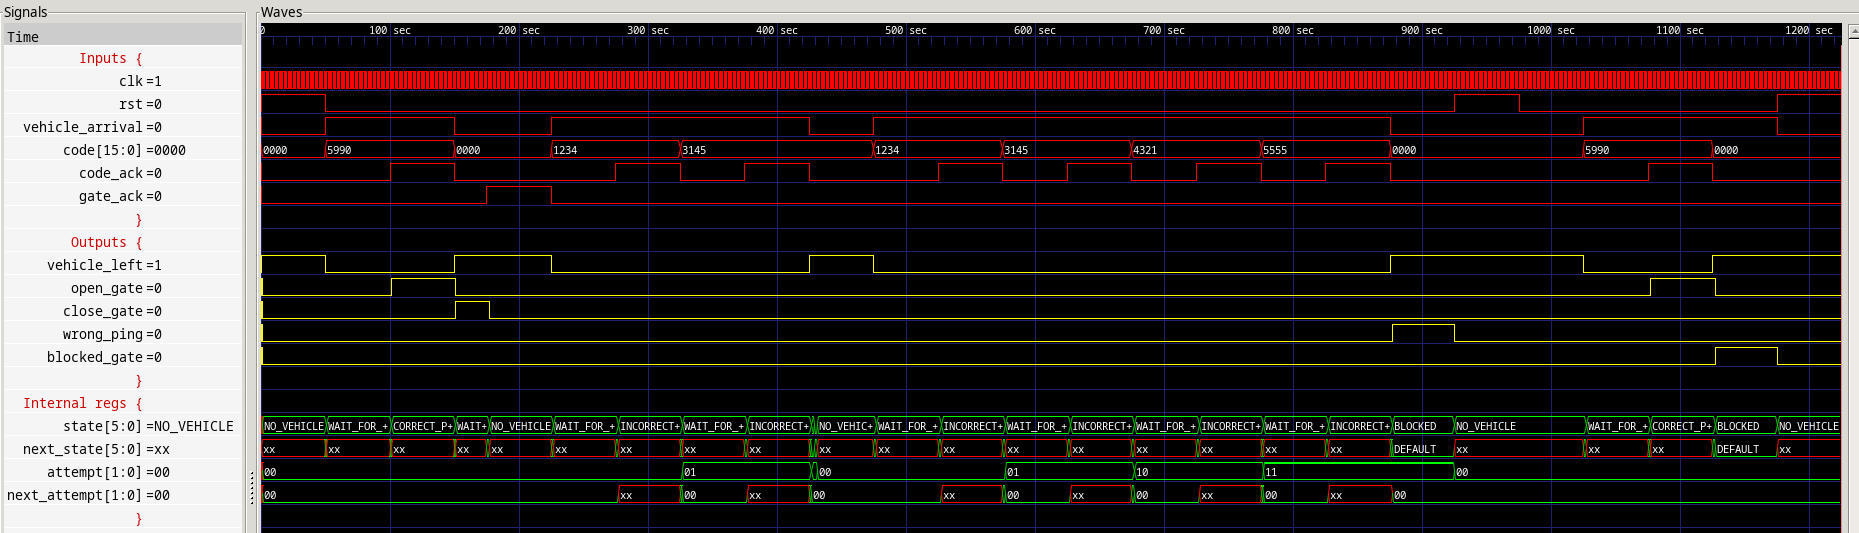
\includegraphics[width = \linewidth]{figs/rtlil.png}
    \caption{Forma de onda correspondiente a la simulación del módulo generado por medio de la síntesis con \code{RTLIL}}
    \label{fig3}
\end{figure}

Como puede notar, se activan las salidas adecuadas en los estados correspondientes y el comportamiento general del módulo es el mismo que el módulo conductual, con la excepción de las condiciones no importa en las variables \code{next\_attempt} y \code{next\_state}. Por tanto, este módulo pasa las 4 pruebas.

\subsection{cmos\_cells.lib}
Se obtuvo la siguiente forma de onda:
\begin{figure}[!h]
    \centering
    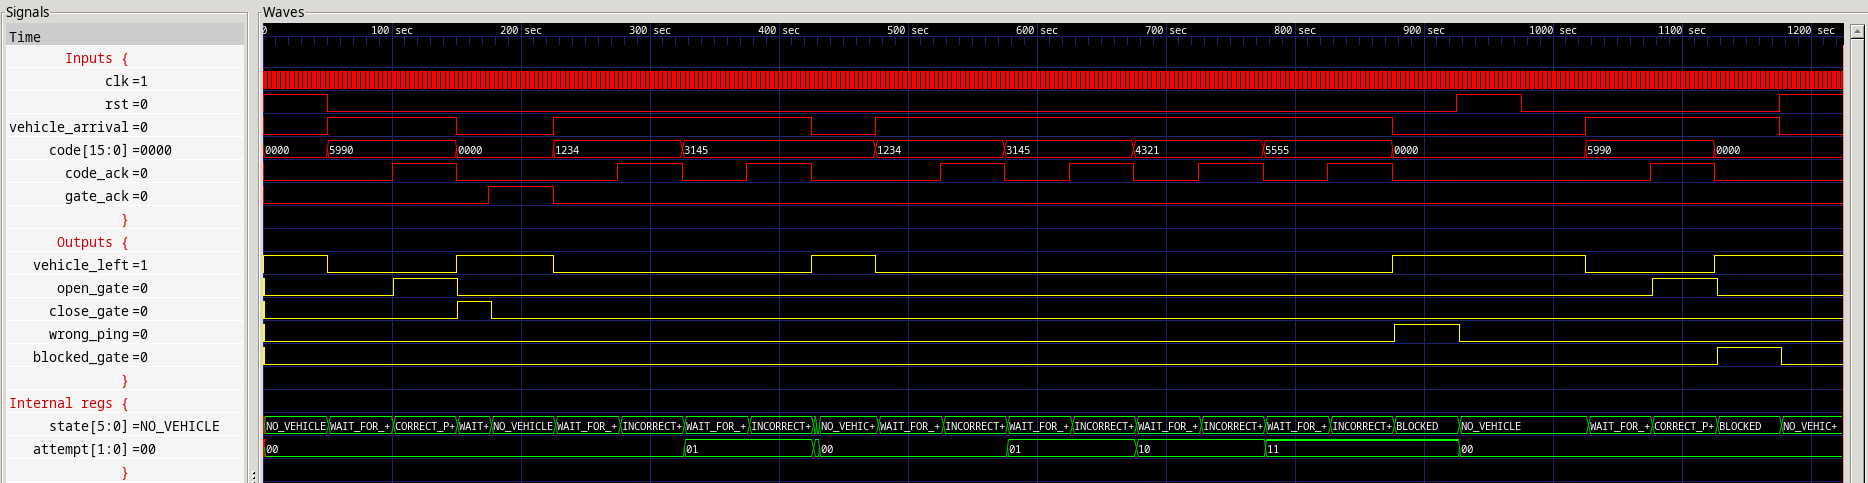
\includegraphics[width = \linewidth]{figs/cmoscells.png}
    \caption{Forma de onda correspondiente a la simulación del módulo generado por medio de la síntesis con \code{cmos\_cells.lib}}
    \label{fig1111}
\end{figure}

Como puede notar, se activan las salidas adecuadas en los estados correspondientes y el comportamiento general del módulo es el mismo que el módulo conductual. Por tanto, este módulo pasa las 4 pruebas.
\newpage

\subsection{cmos\_cells.lib con retardos}
Se obtuvo la siguiente forma de onda:
\begin{figure}[!h]
    \centering
    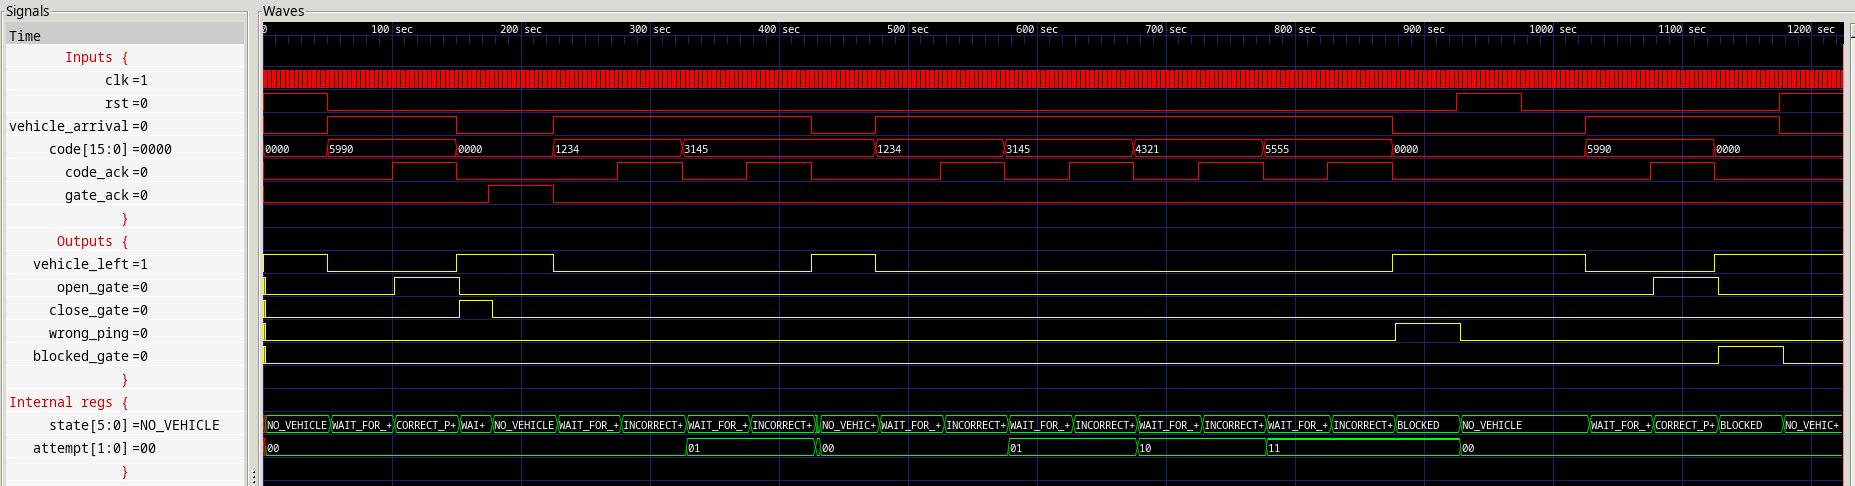
\includegraphics[width = \linewidth]{figs/cmoscellsdelay.png}
    \caption{Forma de onda correspondiente a la simulación del módulo generado por medio de la síntesis con \code{cmos\_cells.lib} con retardos}
    \label{fig111}
\end{figure}

Como puede notar, se activan las salidas adecuadas en los estados correspondientes y el comportamiento general del módulo es el mismo que el módulo conductual. Por tanto, este módulo pasa las 4 pruebas. En la siguiente figura, se muestran dos marcadores para visualizar el retardo entre los estímulos y la respuesta del sistema causado por el retardo añadido a los flip-flops D:

\begin{figure}[!h]
    \centering
    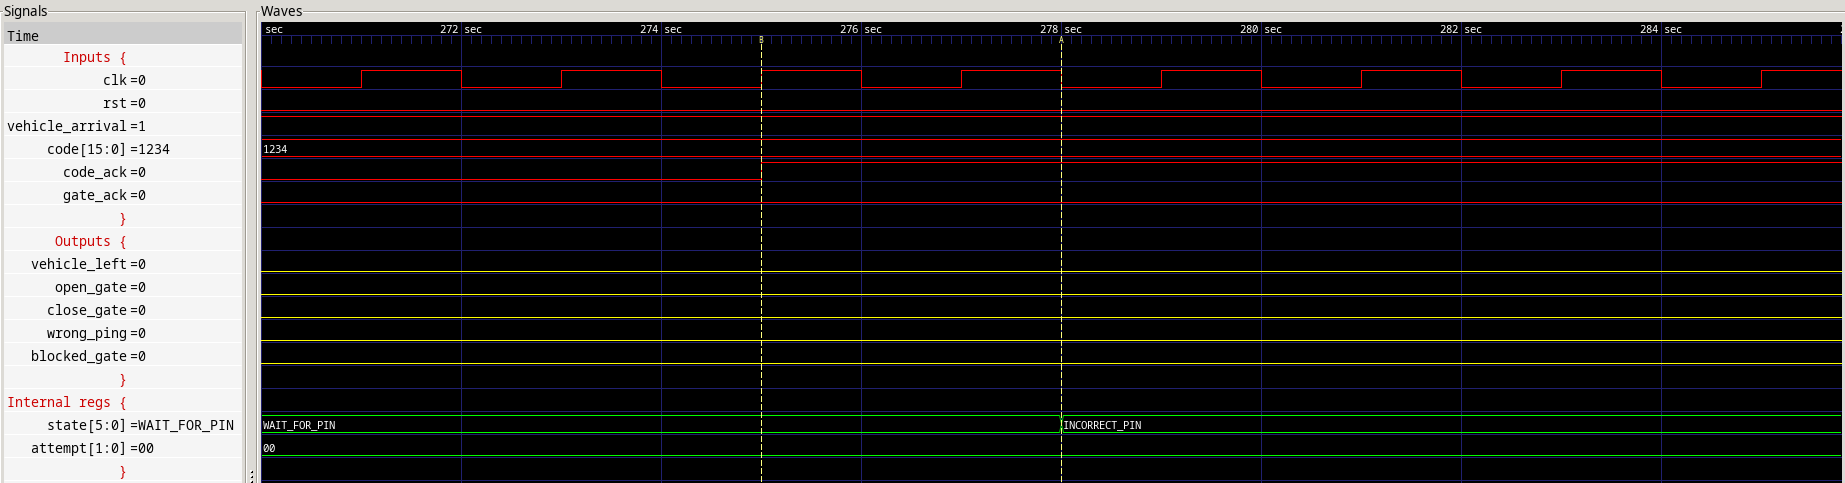
\includegraphics[width = \linewidth]{figs/retardo.png}
    \caption{Visualización de retardo en los flip-flops D del módulo en la forma de onda de la simulación del módulo generado por medio de la síntesis con \code{cmos\_cells.lib} con retardos}
    \label{fig11}
\end{figure}

El tiempo de propragación $\Delta T_{propagacion}$ viene dado por:
\begin{align*}   
    \Delta T_{propagacion}  &= T_{reaccion} - T_{estimulo}\\
                            &= \SI{278}{s} - \SI{275}{s}\\
                            &= \SI{3}{s}
\end{align*}
Note que este tiempo es mayor al que se ajustó en \code{cmos\_cells\_delay.v}.
La razón de esto es debido a que el estímulo es aplicado en un flanco positivo de reloj, por lo que va verse reflejado hasta el siguiente flanco positivo. 
Sin embargo, a causa de que el tiempo de retardo ajustado para los flip-flops D equivale a un semiciclo de la señal \code{clk}, la reacción del sistema va suceder en los flancos negativos en vez de los positivos. Sea $\Delta T_{flanco}$ el tiempo que transcurre desde que se aplica el estímulo y el siguiente flanco de reloj, y $\Delta T_{retardo} = \SI{1}{s}$. Entonces:
\begin{align*}   
    \Delta T_{propagacion}  &= \Delta T_{retardo} + \Delta T_{flanco}\\
\end{align*}
De tal manera de que en el caso expuesto en la figura anterior, $\Delta T_{flanco} = \SI{2}{s}$.
